\section{Meta-Information Extraction for Problem Space Compression}
\label{sec:meta-information-extraction}

This section establishes the mathematical framework for meta-information extraction that analyzes structural information patterns within high-dimensional data spaces, enabling exponential compression of processing complexity through systematic identification of organizational hierarchies and structural redundancies.

\subsection{Meta-Information Mapping Function}

\begin{definition}[Meta-Information Transform]
Let $\mathcal{I}$ represent the information space and $\mathcal{M}$ the meta-information space. The meta-information extraction function $\mu: \mathcal{I} \to \mathcal{M}$ maps information elements to their organizational characteristics:
\begin{equation}
\mu(x) = \langle \alpha(x), \beta(x), \gamma(x), \delta(x), \pi(x) \rangle
\label{eq:meta-information-function}
\end{equation}
where $\alpha(x)$ represents information type classification, $\beta(x)$ semantic density, $\gamma(x)$ connectivity degree, $\delta(x)$ compression potential, and $\pi(x)$ structural patterns.
\end{definition}

\subsection{Information Type Classification}

The information type classifier $\alpha: \mathcal{I} \to [0,1]^4$ decomposes information elements into fundamental organizational categories:

\begin{equation}
\alpha(x) = \langle \alpha_{\text{struct}}(x), \alpha_{\text{rand}}(x), \alpha_{\text{period}}(x), \alpha_{\text{hierarch}}(x) \rangle
\label{eq:info-type-classification}
\end{equation}

For image-based information elements $x \in \mathbb{R}^{H \times W}$:

\begin{align}
\alpha_{\text{struct}}(x) &= \frac{1}{HW} \sum_{i,j} \|\nabla x_{i,j}\| \cdot \mathbf{1}_{\{\|\nabla x_{i,j}\| > \tau_{\text{edge}}\}} \label{eq:structural-score}\\
\alpha_{\text{rand}}(x) &= -\frac{1}{\log K} \sum_{k=1}^K p_k \log p_k \label{eq:randomness-score}\\
\alpha_{\text{period}}(x) &= \frac{1}{HW} \sum_{u,v} \mathbf{1}_{\{|\hat{X}(u,v)| > \tau_{\text{fft}}\}} |\hat{X}(u,v)|^2 \label{eq:periodicity-score}\\
\alpha_{\text{hierarch}}(x) &= \exp\left(-\text{Var}\left(\frac{d\sigma_s^2}{ds}\right)\right) \label{eq:hierarchical-score}
\end{align}

where $\hat{X}(u,v)$ represents the 2D Fourier transform, $p_k$ denotes histogram probability masses, $\sigma_s^2$ represents variance at scale $s$, and $\tau_{\text{edge}}, \tau_{\text{fft}}$ are threshold parameters.

\subsection{Semantic Density Quantification}

\begin{definition}[Local Semantic Density]
The semantic density function $\beta: \mathcal{I} \times 2^{\mathcal{I}} \to [0,1]$ quantifies local information concentration:
\begin{equation}
\beta(x, \mathcal{D}) = \frac{1}{|\mathcal{D}|} \sum_{y \in \mathcal{D}} \exp\left(-\frac{\|f(x) - f(y)\|^2}{2\sigma_{\beta}^2}\right)
\label{eq:semantic-density}
\end{equation}
where $f: \mathcal{I} \to \mathbb{R}^d$ represents a feature extraction mapping and $\sigma_{\beta} > 0$ controls the locality radius.
\end{definition}

For high-dimensional spaces, the feature mapping employs dimensionality reduction:

\begin{equation}
f(x) = \text{PCA}_k(x) = \mathbf{U}_k^T (x - \bar{x})
\label{eq:feature-mapping}
\end{equation}

where $\mathbf{U}_k \in \mathbb{R}^{n \times k}$ contains the first $k$ principal components and $\bar{x}$ denotes the sample mean.

\subsection{Structural Connectivity Analysis}

\begin{definition}[Connectivity Degree]
The structural connectivity degree $\gamma: \mathcal{I} \times 2^{\mathcal{I}} \to [0,1]$ measures the proportion of significant connections:
\begin{equation}
\gamma(x, \mathcal{D}) = \frac{1}{|\mathcal{D}| - 1} \sum_{y \in \mathcal{D} \setminus \{x\}} \mathbf{1}_{\{\rho(x,y) > \tau_{\text{conn}}\}}
\label{eq:connectivity-degree}
\end{equation}
where $\rho(x,y)$ represents a similarity measure and $\tau_{\text{conn}} \in (0,1)$ defines the connectivity threshold.
\end{definition}

The connectivity graph $\mathcal{G} = (\mathcal{V}, \mathcal{E})$ with vertices $\mathcal{V} = \mathcal{D}$ and edges $\mathcal{E} = \{(x,y) : \rho(x,y) > \tau_{\text{conn}}\}$ enables network-theoretic analysis:

\begin{equation}
\text{ClusteringCoeff}(x) = \frac{2e_x}{k_x(k_x - 1)}
\label{eq:clustering-coefficient}
\end{equation}

where $e_x$ represents the number of edges between neighbors of $x$ and $k_x = |\{y : (x,y) \in \mathcal{E}\}|$ denotes the degree of vertex $x$.

\subsection{Compression Potential Estimation}

\begin{definition}[Compression Potential Coefficient]
The compression potential $\delta: \mathcal{I} \times [0,1]^4 \times [0,1]^2 \to [0,1]$ estimates achievable compression ratios:
\begin{equation}
\delta(x, \alpha(x), \beta(x), \gamma(x)) = w_1 \alpha_{\text{struct}}(x) + w_2 \alpha_{\text{hierarch}}(x) + w_3 \beta(x) + w_4 \gamma(x)
\label{eq:compression-potential}
\end{equation}
where $\{w_i\}_{i=1}^4$ represent learned weighting coefficients with $\sum_{i=1}^4 w_i = 1$.
\end{definition}

The weighting coefficients optimize compression prediction accuracy through empirical risk minimization:

\begin{equation}
\mathbf{w}^* = \arg\min_{\mathbf{w}} \sum_{j=1}^N \left( \delta(x_j; \mathbf{w}) - \frac{|x_j|}{|C(x_j)|} \right)^2 + \lambda \|\mathbf{w}\|_2^2
\label{eq:weight-optimization}
\end{equation}

where $C(x_j)$ represents the compressed representation of $x_j$ and $\lambda > 0$ provides regularization.

\subsection{Structural Pattern Extraction}

\begin{definition}[Structural Pattern Space]
The structural pattern extraction function $\pi: 2^{\mathcal{I}} \to \mathcal{P}$ maps datasets to pattern spaces:
\begin{equation}
\pi(\mathcal{D}) = \{\pi_{\text{cluster}}(\mathcal{D}), \pi_{\text{pca}}(\mathcal{D}), \pi_{\text{graph}}(\mathcal{D})\}
\label{eq:structural-patterns}
\end{equation}
\end{definition}

The clustering pattern $\pi_{\text{cluster}}(\mathcal{D})$ employs k-means analysis:

\begin{align}
\pi_{\text{cluster}}(\mathcal{D}) &= \arg\min_{\{\mathbf{c}_k\}_{k=1}^K} \sum_{k=1}^K \sum_{x \in C_k} \|x - \mathbf{c}_k\|^2 \label{eq:kmeans-objective}\\
\text{where } C_k &= \{x \in \mathcal{D} : k = \arg\min_{j} \|x - \mathbf{c}_j\|\} \label{eq:cluster-assignment}
\end{align}

The principal component pattern $\pi_{\text{pca}}(\mathcal{D})$ identifies dominant variation directions:

\begin{equation}
\pi_{\text{pca}}(\mathcal{D}) = \text{eig}\left(\frac{1}{|\mathcal{D}|} \sum_{x \in \mathcal{D}} (x - \bar{x})(x - \bar{x})^T\right)
\label{eq:pca-pattern}
\end{equation}

\subsection{Compression Ratio Quantification}

\begin{theorem}[Compression Ratio Bound]
For a dataset $\mathcal{D}$ with meta-information $\{\mu(x_i)\}_{i=1}^N$, the achievable compression ratio satisfies:
\begin{equation}
C_{\text{ratio}}(\mathcal{D}) \geq 1 + \left(\frac{1}{N} \sum_{i=1}^N \delta(x_i)\right) \cdot (C_{\max} - 1)
\label{eq:compression-ratio-bound}
\end{equation}
where $C_{\max}$ represents the theoretical maximum compression ratio for perfectly structured data.
\end{theorem}

\begin{proof}[Sketch]
The bound follows from the convexity of compression functions and Jensen's inequality applied to the compression potential coefficients. The linear relationship emerges from the weighted combination structure in Equation~\eqref{eq:compression-potential}.
\end{proof}

\subsection{Algorithmic Implementation and Complexity}

The meta-information extraction algorithm processes datasets through parallel analysis:

\begin{algorithm}[H]
\caption{Meta-Information Extraction}
\begin{algorithmic}[1]
\STATE Input: Dataset $\mathcal{D} = \{x_i\}_{i=1}^N$
\FOR{$i = 1$ to $N$}
    \STATE Compute $\alpha(x_i)$ via Equations~\eqref{eq:structural-score}--\eqref{eq:hierarchical-score}
    \STATE Calculate $\beta(x_i, \mathcal{D})$ via Equation~\eqref{eq:semantic-density}
    \STATE Determine $\gamma(x_i, \mathcal{D})$ via Equation~\eqref{eq:connectivity-degree}
    \STATE Estimate $\delta(x_i)$ via Equation~\eqref{eq:compression-potential}
\ENDFOR
\STATE Extract $\pi(\mathcal{D})$ via Equations~\eqref{eq:kmeans-objective}--\eqref{eq:pca-pattern}
\STATE Compute $C_{\text{ratio}}(\mathcal{D})$ via Equation~\eqref{eq:compression-ratio-bound}
\STATE Return $\{\mu(x_i)\}_{i=1}^N, \pi(\mathcal{D}), C_{\text{ratio}}(\mathcal{D})$
\end{algorithmic}
\end{algorithm}

The computational complexity scales as $\mathcal{O}(N^2 d + N d^2 + k^3)$ where $N$ represents dataset size, $d$ dimensionality, and $k$ the number of principal components retained. The quadratic term emerges from pairwise similarity computations, while the cubic term results from eigenvalue decomposition.

This meta-information extraction framework enables systematic identification of compressible structures within high-dimensional information spaces, providing the foundational mechanism for exponential complexity reduction in cognitive processing architectures.

\begin{figure}[htbp]
\centering
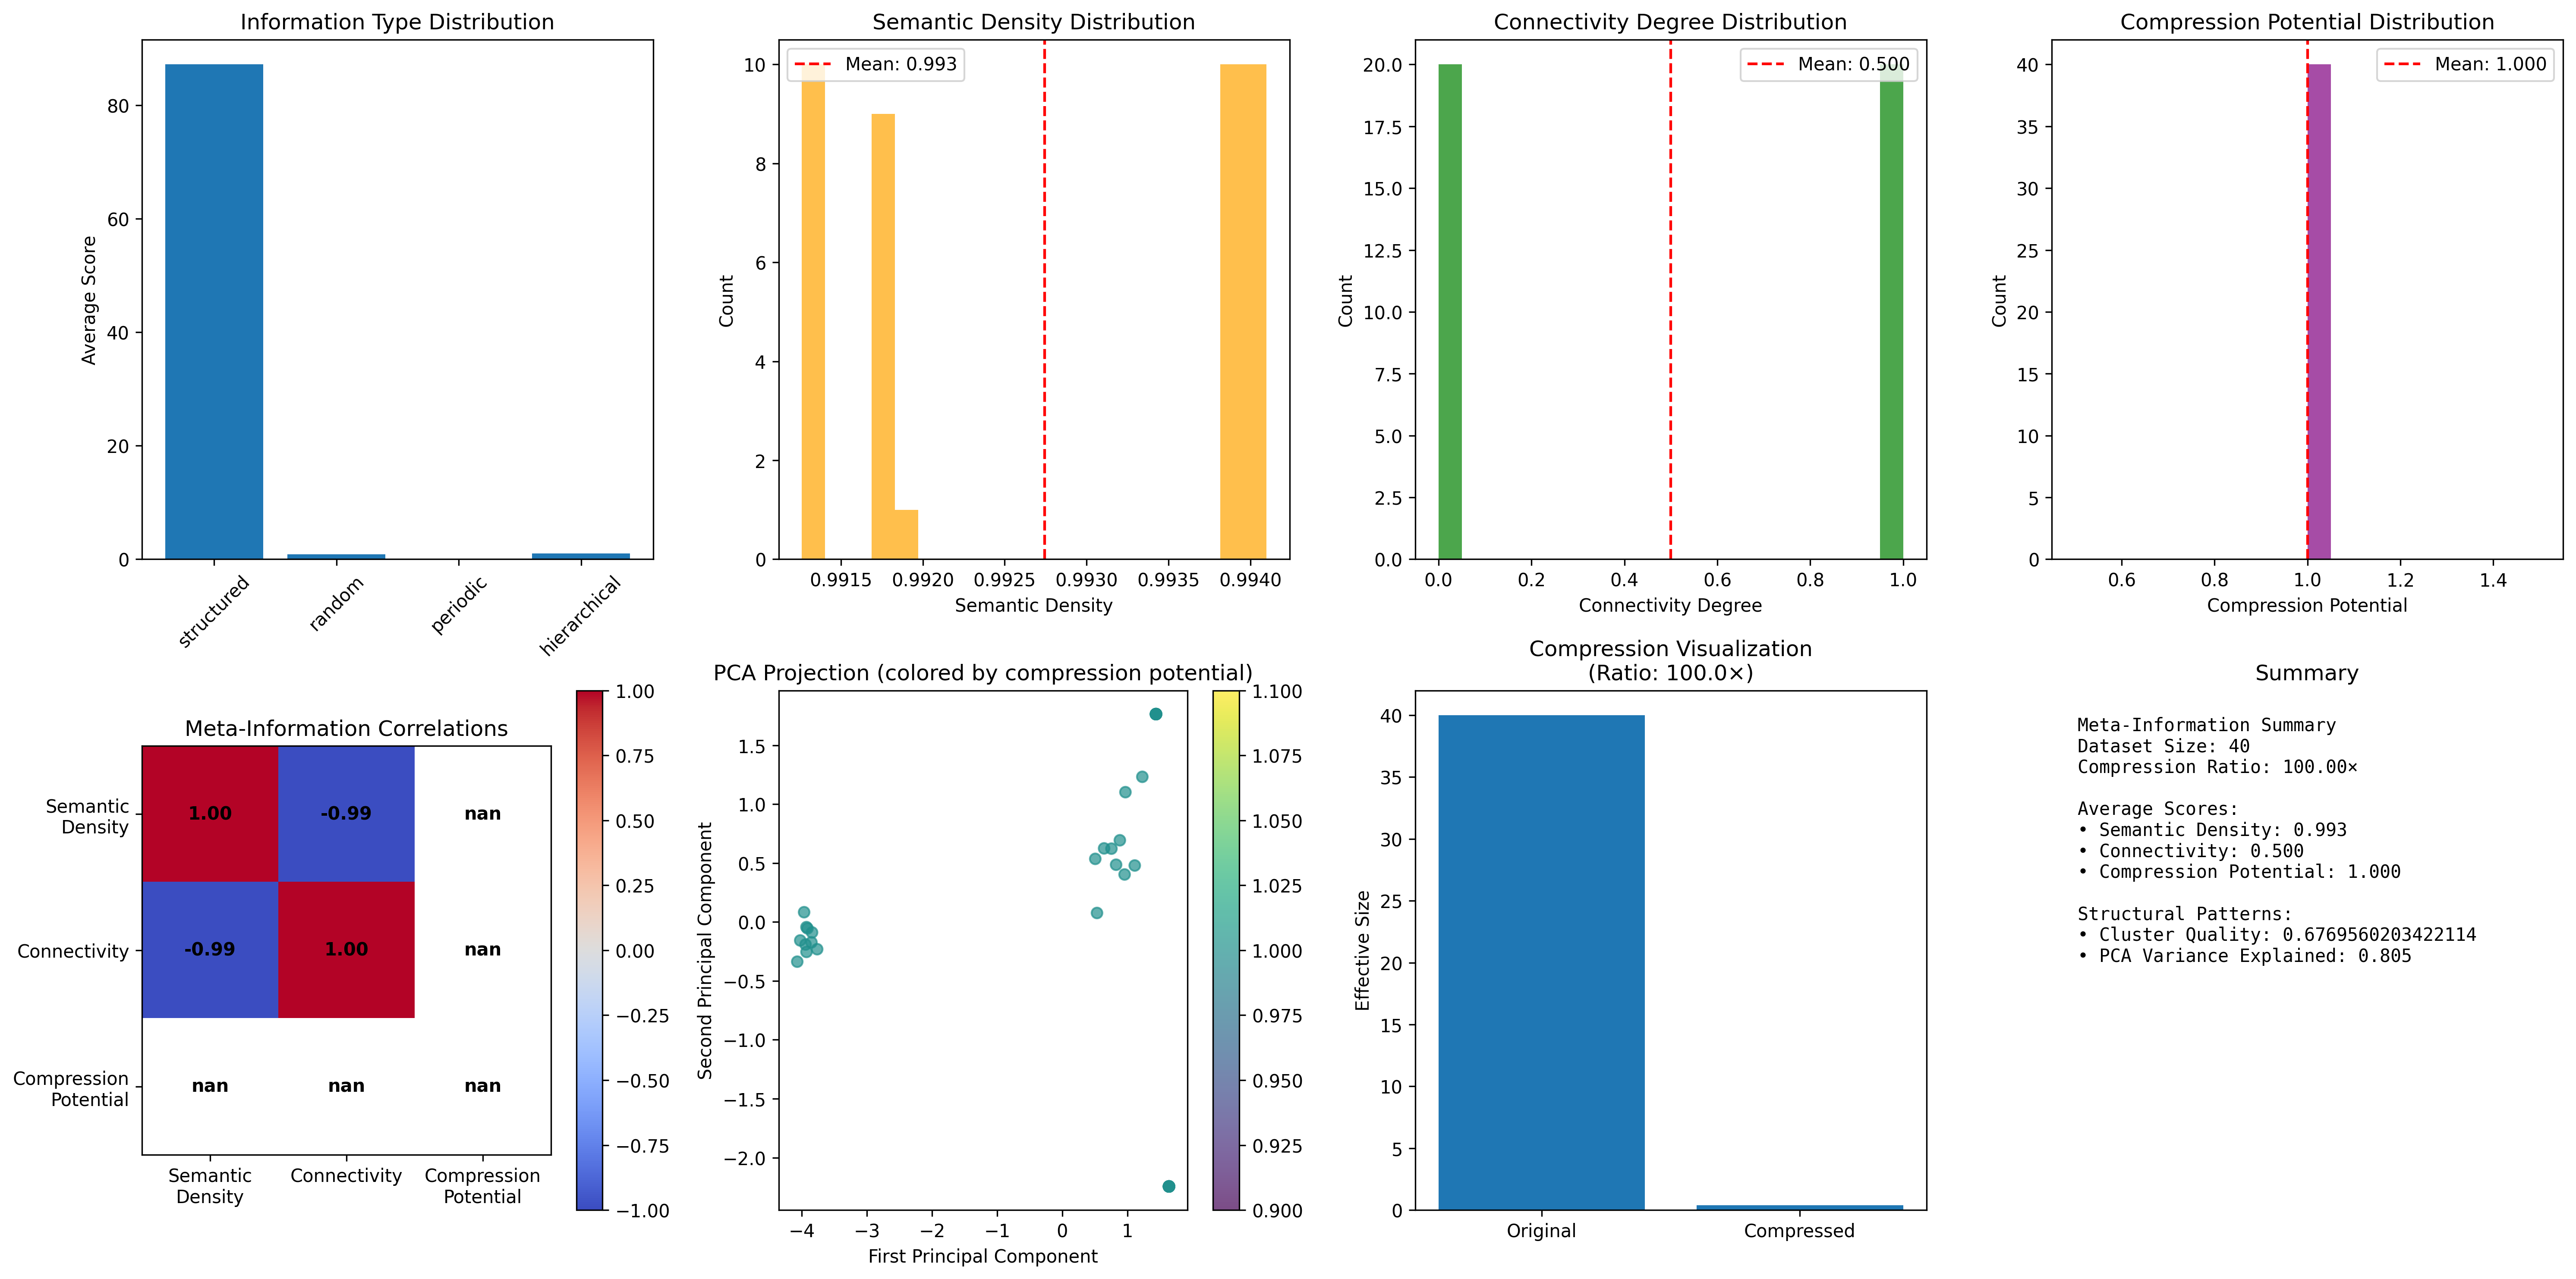
\includegraphics[width=\textwidth]{images/meta_information_extraction_demo.png}
\caption{\textbf{Meta-Information Extraction Analysis.} Comprehensive visualization of structural pattern identification showing: (top row) information type distributions across structured, random, periodic, and hierarchical categories; semantic density, connectivity degree, and compression potential distributions; (bottom row) correlation matrix between meta-information dimensions, PCA projection colored by compression potential, compression ratio visualization comparing original versus compressed effective sizes, and complete meta-information summary statistics. The analysis demonstrates systematic identification of compressible structures enabling exponential complexity reduction through structural pattern recognition.}
\label{fig:meta-information-extraction}
\end{figure}
